%----------- Capítulo 4: Metodologia --------------

\chapter{Metodologia}
\label{metod}

% TODO: escrever uma breve introdução do capítulo
% TODO: devemos falar da IDE usada? e do Jetty?
% TODO: falar sobre convenções de estilo de código?
% TODO: talvez falar um pouco sobre integração contínua em algum canto:
% http://en.wikipedia.org/wiki/Continuous_integration

Com a especificação e uma arquitetura inicial do \emph{software} já estabelecidas, o passo seguinte foi dar início à fase de implementação do produto.
Porém antes deste passo é necessário definir o processo que será utilizado durante a codificação, como será feita a alocação de tarefas entre os membros da equipe, a definição de metas, assim como qual o processo utilizado para garantir a qualidade do sistema que está sendo desenvolvido.

Este capítulo é dividido em duas seções principais: a primeira procura descrever o processo de desenvolvimento de \emph{software} estabelecido pela equipe, enquanto que a segunda apresenta as ferramentas utilizadas durante a fase de implementação.


\section{Processo de Desenvolvimento do \emph{Software}}

Tendo em vista que a equipe foi composta por apenas três integrantes, foi adotado um processo de desenvolvimento de \emph{software} inspirado em Métodos Ágeis, prezando mais pela simplicidade e por um \emph{software} funcional do que uma documentação extensa.

Para garantir a funcionalidade do \emph{software}, foram periodicamente estabelecidas \emph{milestones} (ou metas) através de reuniões da equipe, cada uma destas correspondendo à uma funcionalidade específica do \emph{software}.
Além disso, estas reuniões foram utilizadas para analisar a qualidade do código que havia sido escrito até então, em um processo chamado de \emph{code review} (ou revisão de código), bem como o cumprimento das \emph{milestones} previamente estabelecidas.
Ao estabelecer novas metas, cada integrante da equipe se responsabilizava por um sub-conjunto destas, de forma que cada um desenvolva uma parte do \emph{software} que seja, de preferência, do seu interesse.

Para assegurar a qualidade do código escrito, foram utilizadas, além do processo de \emph{code review}, ferramentas de desenvolvimento orientado a testes e de cobertura dos testes, as quais são discutidas em maiores detalhes na seção a seguir.

\subsection{Desenvolvimento Orientado a Testes}

Para reforçar a ideia de qualidade do código do \emph{software}, minimizar os \emph{bugs} e manter a simplicidade do código, optou-se por utilizar uma adaptação do processo de desenvolvimento de \emph{software} orientado a testes.

Como mencionado na seção \ref{fun:tdd}, o processo de desenvolvimento de \emph{software} orientado a testes baseia-se na repetição de um pequeno ciclo: inicialmente os desenvolvedores escrevem casos de teste nos quais o \emph{software} falha, em seguida o código para que o \emph{software} passe nos novos testes é escrito e, por fim, o código é refatorado para adequar-se aos padrões do projeto.

Neste projeto, a equipe optou por adaptar este método, de forma que não seja obrigatório escrever os casos de teste antes das funcionalidades do \emph{software}, acelerando o processo de desenvolvimento.
No entanto, todo código escrito deve ser testado adequadamente antes de ser enviado ao sistema de controle de versão, com o objetivo de evitar que \emph{bugs} sejam introduzidos no código versionado.

O processo orientado a testes também permitiu que a equipe desenvolvesse o \emph{software} em passos menores sem sacrificar a eficiência do grupo.
Os programadores apenas tinham que se preocupar em cumprir as metas propostas na última reunião e garantir que o código passasse nos testes, focando muito mais no desenvolvimento do código em si e nas funcionalidades desejadas do projeto.

Os casos de testes foram desenvolvidos por todos os membros da equipe, ou seja, não necessariamente por aqueles que desenvolveram uma determinada funcionalidade que seria testada pelos casos de teste em questão.
Este tipo de abordagem aumenta a confiabilidade dos mesmos, fazendo com que tanto o \emph{software} quanto os testes tenham sido analisados por mais de uma pessoa, diminuindo a probabilidade de que erros surjam neste processo.


\subsubsection{Cobertura dos Testes}

Como na metodologia de TDD os testes são usualmente escritos antes do código do \emph{software}, não existe código escrito que não seja necessário para passar um teste.
Desta forma, os testes resultantes deste processo acabam sempre, invariavelmente, aproximando-se de 100\% de cobertura de código durante os testes.
Ou seja, durante a execução dos testes, praticamente todo o código é percorrido pelos mesmos.

Devido à adaptação feita pela equipe à metodologia de desenvolvimento orientado a testes, a não-obrigatoriedade de escrever os testes antes do código, tornou-se necessária a utilização de uma métrica para analisar se os casos de teste escritos cobrem a maior parte do código escrito possível, com o objetivo de assegurar a qualidade dos testes.

Para analisar a cobertura dos testes escritos, a ferramenta \emph{Cobertura} foi utilizada, a qual é discutida em maiores detalhes na seção \ref{met:Cobertura}.


\subsection{Revisão de Código}

% TODO: citar wikipedia aos montes nessa seção

O processo de revisão de código é a examinação sistemática do código-fonte de um programa.
Este tem o objetivo de encontrar e corrigir erros cometidos durante o desenvolvimento, melhorando tanto a qualidade do \emph{software} quanto as habilidades e conhecimentos dos programadores da equipe.

Os processos que podem ser utilizados para revisão de código encaixam-se em três categorias principais: programação em pares, revisão de código formal e a revisão de código leve.

A programação em pares, amplamente utilizada pelos métodos ágeis, corresponde à um conjunto de técnicas na quais dois programadores trabalham em uma única estação de trabalho: um dos programadores, o \emph{driver}, escreve o código, enquanto o outro, denominado \emph{observer}, revisa cada linha de código digitada.
Apesar de uma tarefa de programação ser concluída mais rapidamente quando dois programadores colaboram, estas técnicas possuem a desvantagem de aumentar o tempo total para o desenvolvimento do \emph{software}. % TODO: justificar isso
Sendo assim, em uma equipe com menos integrantes como é o caso desta, o processo como um todo tornaria-se mais ineficiente, a equipe demoraria mais tempo para concluir o projeto e, por este motivo, a programação em pares foi descartada.

As técnicas de revisão de código formais são o método mais tradicional de revisão de código.
Estas envolvem um detalhado processo com múltiplos participantes e múltiplas fases, sendo o mais comum uma série de reuniões nas quais os desenvolvedores revisam o código linha por linha, geralmente utilizando cópias impressas.
Apesar de exigirem um grande investimento de tempo, tanto para a organização e planejamento quanto para a execução, as técnicas de revisão de código formais são consideradas efetivas para encontrar problemas na codificação.

Por fim, as técnicas de revisão de código leves possuem um \emph{overhead} menor que as inspeções formais e são geralmente conduzidas como parte normal do processo de desenvolvimento de \emph{software}.
Entre os principais exemplos deste tipo de técnica está a revisão de código auxiliada por ferramenta, na qual autores e revisores de código utilizam ferramentas especializadas para \emph{peer code review}, ou seja, revisão de código por pares.

Tendo em vista o tamanho da equipe, optou-se por utilizar a técnica de revisão de código auxiliada por ferramenta, sendo que após cada \emph{commit} no sistema de controle de versões todos os integrantes da equipe analisavam o que foi desenvolvido, fazendo comentários a respeito, sugerindo modificações e discutindo as decisões tomadas.
Além da revisão de código após os \emph{commits}, as reuniões da equipe também foram utilizadas para revisar o código escrito antes de um grande refatoramento no código do projeto ou de dar início ao desenvolvimento de uma nova importante funcionalidade do \emph{software}.

Para o processo de revisão de código, foi utilizado o serviço de hospedagem de projetos de desenvolvimento de \emph{software} GitHub, o qual conta com uma ferramenta de \emph{code review} que será apresentada em maiores detalhes na seção \ref{met:git}.


\section{Ferramentas Utilizadas}

Diversas ferramentas mostraram-se necessárias durante a codificação: que vão desde as linguagens de programação que foram utilizadas no desenvolvimento do sistema, o Sistema Gerenciador de Banco de Dados utilizado para armazenar as informações pertinentes ao domínio do problema e o sistema de controle de versão utilizado para gerenciar o código-fonte desenvolvido, entre outras.
As seções a seguir procuram justificar cada uma das decisões tomadas, bem como apresentar cada uma das ferramentas escolhidas pela equipe.

\subsection{Linguagens de Programação}

Para os componentes do sistema que residem no servidor, ou seja, Core, GTFS Importer e Web Service, a equipe inicialmente optou por escolher uma linguagem de programação que todos os integrantes tivessem conhecimento e alguma experiência, para que não fosse necessário aprender uma nova linguagem, podendo então focar o tempo no aprendizado de outras ferramentas como SGBDs NoSQL e no desenvolvimento do código em si.
Desta forma, as linguagens que foram consideradas para este projeto foram: C++, Java e Python.

% TODO: colocar uma tabela comparativa das linguagens C++, Java e Python

A linguagem C++ foi criada por Bjarne Stroustrup em 1979 no Bell Labs.
Originalmente, esta foi criada como uma extensão que insere diversas funcionalidades à linguagem C, tais como classes, sobrecarga de operadores, herança múltipla, \emph{templates} e tratamento de exceções.
Atualmente, C++ é uma das linguagems mais populares, com domínios de aplicações que incluem sistemas operacionais, aplicativos para \emph{desktops}, \emph{drivers} para dispositivos de hardware, sistemas embarcados e aplicações de servidores e clientes que exigem alta performance.
% TODO: talvez falar um pouco sobre a performance de C++ ser bem melhor que a de Python e Java

O principal motivo pelo qual a equipe optou por descartar a linguagem C++ foi a ausência de um sistema de \emph{garbage collection}, o que torna mais difícil a manutenção da base de código e aumenta a probabilidade de erros de programação relacionados com \emph{memory leaks} (ou ``vazamentos de memória''), que são um problema comum quando uma porção de memória alocada para uma determinada operação não é liberada quando não é mais necessária.
Além disso, ao contrário da linguagem C++, as linguagens Java e Python possuem ferramentas para desenvolvimento de aplicações web amplamente utilizadas e documentadas, como os \emph{frameworks} Django e Pylons da linguagem Python e a plataforma J2EE da linguagem Java.

A linguagem Python, por sua vez, foi criada por Guido van Rossum no fim da década de 80, sendo que a primeira implementação do interpretador CPython, a implementação referência da linguagem, começou a ser desenvolvida em Dezembro de 1989.
A filosofia desta linguagem enfatiza a legibilidade do código, reforçando uma sintaxe clara e de fácil entendimento até mesmo para aqueles que não conhecem a linguagem.
Python também possui uma biblioteca padrão bastante completa, que é considerada como um de seus pontos mais fortes, com módulos que vão desde aritmética com precisão arbitrária até expressões regulares, interfaces com bancos de dados relacionais e execução de testes unitários.

A linguagem Java foi criada por James Gosling enquanto trabalhava na Sun Microsystems.
Lançada em 1995 como um dos principais componentes da plataforma Java, a linguagem teve sua sintaxe inspirada na de C++, compartilhando diversas características com a mesma.
Ao contrário de C++, os aplicativos desenvolvidos em Java são compilados na forma de \emph{bytecode} e podem, portanto, ser executados em qualquer computador que possua uma máquina virtual Java instalada, independente de arquitetura ou sistema operacional.
Assim como Python, a linguagem Java possui uma extensa biblioteca padrão, também contando com módulos para acesso à bancos de dados relacionais, \emph{toolkits} para a confecção de interfaces gráficas, \emph{sockets}, \emph{threads}, entre outros.
Outra vantagem da linguagem Java são os Servlets: classes Java que estendem as funcionalidades de servidores que hospedam aplicações acessadas por meio de requisições e respostas.
Apesar de poderem ser utilizadas para responder qualquer tipo de requisição, os Servlets são geralmente utilizados para estender aplicações hospedadas por servidores Web e, sendo assim, de grande utilidade para este projeto.

A decisão pela linguagem de programação a ser utilizada nas componentes da aplicação presentes no servidor foi influenciada em grande parte pela decisão do Sistema Gerenciador de Banco de Dados do projeto.
Como é apresentado na Tabela \ref{tab:bancos}, os principais SGBDs NoSQL existentes são escritos em linguagem Java e, sendo assim, todos estes possuem \emph{bindings} para esta.
Além disso, os integrantes da equipe possuíam conhecimentos prévios de linguagem Java, assim como construção de Servlets.
Somando-se estes pontos à extensa documentação fornecida pela linguagem, optou-se por utilizá-la nas aplicações do servidor.

Com relação ao cliente Web, foram consideradas duas opções: a primeira seria desenvolver este utilizando a linguagem Java, sob a forma de um Applet Java, enquanto que a segunda seria utilizar apenas utilizar páginas em HTML simples com o auxílio de JavaScript para melhorar a experiência do usuário.

A principal desvantagem de se utilizar Applets Java para a interface do cliente Web é a necessidade do usuário ter uma implementação da máquina virtual Java instalada em seu computador para utilizar o sistema.
Além disso, devido ao \emph{overhead} imposto pela máquina virtual, os Applets Java tendem a demorar mais tempo para carregar no navegador Web, prejudicando a experiência do usuário.
Sendo assim, esta opção foi descartada pela equipe e optou-se por desenvolver o cliente Web utilizando apenas páginas HTML e JavaScript.

A linguagem JavaScript foi desenvolvida por Brendan Eich durante a década de 90, enquanto trabalhava na Netscape.
Apesar do nome, a linguagem não possui grande relação com Java, excetuando-se o fato de que aquela foi influenciada por esta em alguns aspectos como, por exemplo, as convenções de nome e a de sintaxe.
Atualmente, JavaScript é amplamente utilizada para o desenvolvimento de interfaces de usuário para a \emph{Web} e \emph{websites} dinâmicos.

Com o crescimento da demanda por aplicações escritas em JavaScript, uma série de bibliotecas para facilitar o desenvolvimento deste tipo de aplicação surgiu.
Entre estas destaca-se a biblioteca jQuery que, por ser a mais popular, contém uma extensa documentação e diversas funcionalidades, que vão desde efeitos e animações, até manipulação de folhas de estilo e métodos para comunicação assíncrona com servidores de aplicações Web.
Por estes motivos, optou-se por utilizar também esta biblioteca para o desenvolvimento do cliente Web.

\subsection{Sistema Gerenciador de Banco de Dados}

% TODO: falar algo do Neo4j spatial

Como citado anteriormente, os SGBDs NoSQL permitem que os dados sejam armazenados de uma forma menos rígida que nos bancos de dados relacionais.
Por este motivo, os bancos de dados NoSQL apresentam uma grande vantagem com relação aos demais para armazenar e extrair informações rapidamente de bases de dados que possam ser modeladas como grafos. % TODO: citar algo

Dada a natureza do problema sendo estudado, naturalmente a equipe optou por utilizar um dos bancos de dados NoSQL que enfatizam em grafos.
Entre as principais opções disponíveis que foram consideradas para este projeto estão o HyperGraphDB, desenvolvido pela Kobrix Software Inc., o InfoGrid, desenvolvido pela NetMesh Inc., o Neo4j, desenvolvido pela Neo Technology Inc. e o OrientDB, desenvolvido pela Orient Technologies.
Estes bancos de dados são apresentados na Tabela \ref{tab:bancos}.

Outros bancos de dados disponíveis na Internet também foram inicialmente analisados, como o FlockDB, desenvolvido pela Twitter Inc..
No entanto, estes foram desconsiderados posteriormente por não possuírem documentação suficiente no momento em que foi dado início ao desenvolvimento do projeto ou focarem demais em um problema específico, como é o caso do próprio FlockDB, que é utilizado para armazenar as relações sociais entre os usuários do serviço do Twitter: ``quem segue quem'' e ``quem é seguido por quem''.

\begin{table}[!htb]
	\centering
	\caption{Tabela comparativa entre as opções de SGBDs disponíveis}
	\label{tab:bancos}
	\begin{tabular}{lcccc}
		\hline
		& \textbf{HyperGraphDB} & \textbf{InfoGrid} & \textbf{Neo4j} & \textbf{OrientDB} \\
		\hline
		\textbf{Licença} & LGPL & AGPLv3 & AGPLv3 & Apache \\
		\textbf{Iniciado em} & 2005 & ? & 2003 & ? \\
		\textbf{Versão estável} & 1.1 & 2.9.5 & 1.4.2 & 0.9.25 \\
		\textbf{Data versão estável} & Dezembro 2010 & Agosto 2011 & Setembro 2011 & Março 2011 \\
		\textbf{Bindings Java} & Sim & Sim & Sim & Sim \\
		\textbf{Bindings Python} & Não & Não & Sim & Parcial \\
		\textbf{Bindings C/C++} & Não & Não & Não & Não \\
		\textbf{Stand-alone} & Sim & ? & Sim & Sim \\
		\textbf{Embarcado} & Não & ? & Sim & Sim \\
		\textbf{Suporte Blueprints} & Não & Não & Sim & Sim \\
		\hline
	\end{tabular}
	\fonte{Autoria pr\'opria.}
\end{table}

Entre os SGBDs apresentados na Tabela \ref{tab:bancos}, todos são desenvolvidos em linguagem Java e, portanto rodam em qualquer plataforma que possua uma implementação da \sigla{JVM}{Java Virtual Machine}.
Além disso, todos eles são disponibilizados através de uma licença de \emph{software} livre.
No entanto, os bancos de dados InfoGrid e Neo4j são também distribuídos através de licenças comerciais, sendo a versão livre destes uma versão com menos funcionalidades e sob uma licença, a \sigla{AGPLv3}{Affero General Public License Version 3}, que impede o desenvolvedor de não disponibilizar o código-fonte de um \emph{software} que utilize o banco de dados. % TODO: verificar se isso que eu falei da AGPLv3 ta certo

Todos os bancos de dados que foram levados em consideração para este projeto apresentavam um conjunto de funcionalidades semelhantes.
Como todos são desenvolvidos em Java, todos possuem bindings para a mesma, reforçando então ainda mais a escolha pela linguagem.

Desta forma, os fatores determinantes para a decisão sobre qual banco de dados utilizar acabaram sendo o suporte dado pela comunidade do mesmo, a documentação e quão frequentes são as atualizações do \emph{software}, tendo em vista que aqueles que são mais bem atualizados possuem uma comunidade mais ativa.
O HyperGraphDB foi desconsiderado por não ser atualizado com frequência, dado que sua última versão estável era de Dezembro de 2010, muito anterior com relação às dos demais bancos.

Já a documentação e suporte da comunidade dos bancos OrientDB e Neo4j mostrou-se muito superior à do InfoGrid, tendo em vista que estes possuem um volume maior de emails nas suas listas de discussões e, portanto, uma comunidade mais ativa.

A decisão final de qual banco de dados utilizar ficou, portanto, entre o Neo4j e o OrientDB.
Optou-se pelo Neo4j principalmente devido à facilidade de aprendizado da sua \sigla{API}{Application Programming Interface}, que possui uma notação mais concisa e com uma curva de aprendizagem adequada, na opinião da equipe.
Outro ponto positivo com relação ao Neo4j é que ele é mantido por uma grande comunidade de desenvolvedores desde 2003 e é, portanto, um dos projetos livres pioneiros nesta área.

\subsection{Gerenciamento e Automação de Projetos}

Tendo em vista a arquitetura em módulos proposta para este projeto, mostrou-se interessante o uso de uma ferramenta capaz de facilitar o processo de \emph{build}, ou seja, compilação e integração dos diferentes módulos da aplicação.

Para tanto, optou-se por utilizar o Apache Maven, o qual é uma ferramenta desenvolvida em linguagem Java para facilitar o gerenciamento de projetos nesta e em outras linguagens de programação.

Entre as principais vantagens de se utilizar o Maven para o gerenciamento de um projeto, estão:
\begin{itemize}
	\item Facilita o processo de \emph{build}, compilação e integração dos módulos da aplicação.
	\item Simplifica a resolução de dependências, permitindo que o desenvolvedor apenas especifique de quais bibliotecas ou módulos o projeto depende, deixando o trabalho de fazer \emph{download} das mesmas e de inserir no \emph{classpath} à cargo do Maven.
	\item Permite a execução de testes unitários e de integração no projeto antes de construir um pacote do mesmo.
	\item Facilita o gerenciamento de projetos de grande porte.
	% TODO: citar mais vantagens
\end{itemize}

Os projetos gerenciados pelo Apache Maven são descritos através de uma estrutura denominada \sigla{POM}{Project Object Model} (\emph{Project Object Model}).
Esta estrutura, especificada sob a forma de um documento \sigla{XML}{Extensible Markup Language} denominado \texttt{pom.xml}, fornece à ferramenta todas as informações relativas ao projeto como, por exemplo: o nome do projeto, os desenvolvedores, o tipo de empacotamento utilizado para a aplicação e suas dependências com outros projetos.
Através do POM também é possível configurar todas as fases do processo de compilação, permitindo especificar até mesmo a versão da linguagem Java que será utilizada para compilação ou evitar que seja gerado um pacote da aplicação quando algum dos testes falhar.

Projetos maiores, como é o caso deste, podem ser divididos em diversos módulos, ou sub-projetos, cada um com o seu próprio POM.
Um projeto principal (ou raiz) é criado, através do qual é possível compilar todos os demais módulos com um único comando.
Os POMs dos sub-projetos podem ainda herdar configurações do projeto principal, tornando possível manter uma padronização entre os projetos e sub-projetos da aplicação com facilidade.

Dadas estas características, esta ferramenta mostrou-se ideal para o desenvolvimento deste projeto, tendo em vista a grande variedade de dependências que o compõem, tais como bibliotecas para acesso ao SGBD, serialização e deserialização de dados, assim como os diversos módulos pelos quais a aplicação é composta.

% TODO: talvez seja interessante ampliar essa seção, dando um exemplo de pom.xml, mais detalhes sobre a ferramenta e tal

\subsection{Sistema de Controle de Versão}\label{met:git}

% referencias: http://betterexplained.com/articles/a-visual-guide-to-version-control/
% http://betterexplained.com/articles/intro-to-distributed-version-control-illustrated/
% http://www.infoq.com/articles/dvcs-guide

O gerenciamento e monitoramento de modificações em documentos, programas e outras informações armazenadas como arquivos de computador é conhecido como controle de versão ou, ainda, controle de revisão.

Durante o processo de desenvolvimento de \emph{software}, é comum que múltiplas versões de um mesmo \emph{software} sejam utilizadas em diferentes locais e que os desenvolvedores trabalhem simultaneamente em partes distintas do \emph{software}.
Novas funcionalidades ou até mesmo \emph{bugs} muitas vezes estão presentes apenas em determinadas versões.
Portanto, para organizar o desenvolvimento, bem como facilitar a localização e correção de \emph{bugs}, é de vital importância determinar em quais versões do \emph{software} os problemas ocorrem.
Inclusive, muitas vezes é necessário desenvolver duas ou mais versões do mesmo \emph{software} em paralelo como, por exemplo, uma na qual os problemas sejam corrigidos sem a criação de novas funcionalidades, enquanto que em outra versão novas funcionalidades são inseridas na aplicação, sendo estas comumente denominadas \emph{branch} e \emph{trunk}, respectivamente.

Enquanto os desenvolvedores poderiam simplesmente manter múltiplas cópias das diferentes versões do projeto no sistema de arquivos, este processo é extremamente ineficiente pois muitas versões praticamente idênticas do \emph{software} teriam que ser mantidas, tornando a tarefa de determinar as modificações entre uma versão e outra difícil, tediosa e sujeita à erros.
Por este motivo, diversos sistemas para automatizar o processo de controle de versão surgiram.

Tradicionalmente, os sistemas de controle de versão mais comuns utilizam um modelo centralizado, no qual todas as funções são desempenhadas em um servidor compartilhado por todos os desenvolvedores.
Sistemas como estes vêm sendo utilizados desde a década de 70 e foram considerados padrão na indústria por muitos anos.
Diversos sistemas de controle de versão livres enquadram-se neste modelo como, por exemplo, o \sigla{CVS}{Concurrent Versions System}, lançado em 1990, e o Subversion, lançado em 2004.

% citar a lista de falhas apontadas por http://www.infoq.com/articles/dvcs-guide
Apesar de muito utilizados, os sistemas de controle de versão centralizados possuem algumas falhas, entre elas:

\begin{itemize}
	\item Criar novos \emph{branches} é fácil de ser feito. No entanto, os \emph{merges}, ou mesclagens, não são.
	\item Ferramentas como o Subversion não possuem um histórico ciente dos \emph{merges}, forçando os usuários a monitorarem manualmente quais \emph{branches} já foram mescladas entre si, tornando o processo sujeito à erros e tedioso.
	\item Sistemas centralizados não permitem que modificações sejam compartilhadas entre os usuários sem que estas sejam enviadas ao repositório central.
	\item Algumas ferramentas, como o Subversion, não são capazes de mesclar modificações quando arquivos ou diretórios foram renomeados em um dos \emph{branches}.
	\item Impossibilidade de fazer \emph{commits} enquanto não há acesso ao servidor central.
\end{itemize}

Estes problemas são, em grande parte, solucionados pelos modernos sistemas de controle de versão distribuídos (ou \sigla{DVCS}{Distributed Version Control System}, \emph{Distributed Version Control System}).
% TODO: explicar melhor o que são os DVCS

O primeiro destes sistemas, o BitKeeper, é desenvolvido pela BitMover Inc. e teve sua primeira versão estável disponibilizada para o público em Maio de 2000.
Este tornou-se muito conhecido quando, em 2002, Linus Torvalds decidiu que esta seria a melhor ferramenta para ser utilizada no desenvolvimento do kernel Linux.
Até então, Linus aplicava cada \emph{patch} submetido pela comunidade manualmente.

Em Abril de 2005, a BitMover Inc. anunciou que não iria mais fornecer uma versão gratuita do BitKeeper para a comunidade.
Com isso, apenas os desenvolvedores do Linux que tivessem acesso à uma versão comercial do BitKeeper poderiam ter acesso ao histórico de versões, por exemplo.
Este evento levou à criação do projeto git, pelo próprio Linus Torvalds, que rapidamente substituiu o BitKeeper como sistema de controle de versão do Linux.

Dada a origem dos sistemas de controle de versão distribuídos, é notável a sua importância para muitos \emph{softwares} livres.
Devido à sua característica de distribuir e permitir a colaboração de diversas pessoas em um mesmo projeto com facilidade, estes sistemas são amplamente utilizados pela grande maioria dos projetos livres.

Tendo em vista que este projeto tem como objetivo o desenvolvimento de um \emph{software} livre, que esteja aberto para futuras contribuições de terceiros, optou-se por utilizar um DVCS para o controle de versão do código.

Apesar de outras ferramentas livres existirem, como o Mercurial, o Bazaar e o darcs, a equipe decidiu utilizar o git como sistema de controle de versão.
Os principais motivos pelos quais a equipe optou por este sistema foram:

\begin{itemize}
	\item Todos os membros da equipe já tinham experiência com esta ferramenta, proveniente de projetos anteriores.
	\item É especialmente popular entre projetos de \emph{software} livre, sendo utilizado por vários projetos como Ruby on Rails, WINE, X.org e até mesmo o sistema operacional para dispositivos móveis Android.
	\item Existência de vários \emph{sites} para hospedagem gratuita de projetos de \emph{software} livre na Internet que suportam o git como sistema de controle de versão, tais como o popular GitHub, Gitorious, SourceForge, Google Code e Bitbucket.
\end{itemize}

\subsubsection{Hospedagem do Repositório}

De acordo com uma pesquisa realizada entre os usuários do git em 2010 \cite{gitus2010}, o \emph{site} de hospedagem de repositórios git mais popular é o GitHub, com mais de 77\% dos usuários de git hospedando seus projetos neste.
Atualmente, o serviço conta com mais de um milhão de usuários e dois milhões de projetos hospedados. % TODO: cite

Diversas características destacam o GitHub com relação aos demais serviços de hospedagem, entre as principais estão as suas ferramentas para gerência de projeto:

\begin{itemize}
	\item É possível criar vários times com diferentes tipos de permissões para trabalhar em determinados repositórios, facilitando o controle de quais usuários podem fazer alterações em cada projeto.
	\item Todos os repositórios hospedados no GitHub possuem um sistema de \emph{bug tracking}, o que permite que os desenvolvedores mantenham uma lista dos \emph{bugs} a serem corrigidos, assim como das funcionalidades a serem implementadas.
Este sistema ainda permite a criação e manutenção de \emph{milestones}, tornando-o compatível com o processo proposto para o desenvolvimento do \emph{software}.
	\item O sistema permite que os desenvolvedores façam comentários nos \emph{commits} feitos no repositório ou, até mesmo, em linhas de código.
Esta característica é extremamente importante para o processo de revisão de código, tornando possível com que os membros da equipe, ou até mesmo contribuidores da comunidade, discutam sobre as decisões tomadas diretamente em cima do código.
\end{itemize}

Aliando-se estas características com a popularidade do GitHub, o que poderá auxiliar o projeto a encontrar colaboradores e dar mais visibilidade ao mesmo, a equipe optou por utilizá-lo como \emph{site} para hospedar o desenvolvimento do \emph{software}.

% TODO: talvez colocar uma figura do GitHub e referenciar no texto?


\subsection{Testes e Cobertura de Código}\label{met:Cobertura}

Existem vários \emph{frameworks} para desenvolvimento de testes unitários e de integração para a linguagem Java.
Entre estes, estão o JTiger, desenvolvido por Tony Morris, o TestNG, desenvolvido por Cedric Beust e Alexandru Popescu, e o mais conhecido dos três, JUnit, desenvolvido por Erich Gamma e Kent Beck.

O JUnit é um dos mais antigos e populares \emph{frameworks} disponíveis para a linguagem Java, sendo conhecido pela grande maioria dos programadores que trabalham com esta.
Apesar de ter sido originalmente criado para testar código escrito em Java, diversas extensões do JUnit estão disponíveis para permitir que testes sejam escritos para praticamente qualquer componente de um sistema, desde arquivos XML até código em JavaScript.
A Figura \ref{fig:testes} apresenta um exemplo de resultados da execução de testes JUnit através da \sigla{IDE}{Integrated Development Environment} Netbeans.
\begin{figure}[!htb]
	\centering
	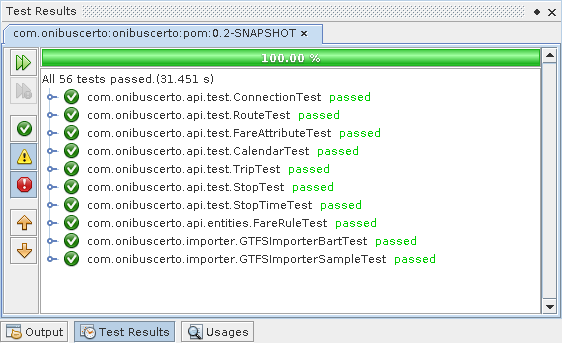
\includegraphics[width=0.6\textwidth]{./imgs/testes.png}
	\caption[Exemplo de execução dos testes]{Exemplo de execução dos testes}
	\fonte{Autoria Própria}
	\label{fig:testes}
\end{figure}

Tendo em vista a compatibilidade do Maven com o JUnit, a popularidade e a familiaridade dos membros da equipe com este, o \emph{framework} foi escolhido como ferramenta para desenvolvimento dos casos de teste.

O uso de uma ferramenta que permita analisar qual a porcentagem de código-fonte do sistema que é coberta pelos testes escritos mostrou-se necessário.
Para tanto, a equipe optou pela ferramenta Cobertura, devido às seguintes características da mesma:

\begin{itemize}
	\item Integração com o Maven através de um \emph{plugin}.
	\item Integração com a IDE Netbeans.
	\item Geração de relatórios em HTML ou XML.
	\item Apresenta nos relatórios a porcentagem de linhas e ramificações cobertas para cada classe, pacote e para o projeto como um todo.
	\item Calcula a complexidade ciclomática de cada classe, assim como a complexidade ciclomática média para cada pacote e para o projeto.
\end{itemize}

Os relatórios gerados por esta ferramenta são de grande importância para identificar com facilidade quais partes do \emph{software} não possuem testes.
Um exemplo de relatório desta ferramenta é apresentado na Figura \ref{fig:cobertura}.

\begin{figure}[!htb]
	\centering
	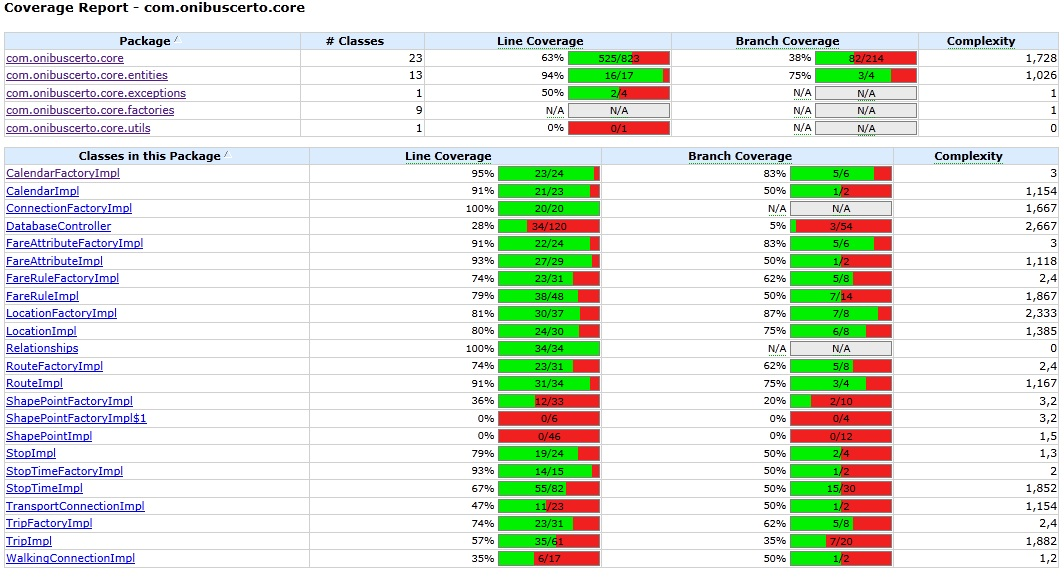
\includegraphics[width=0.8\textwidth]{./imgs/cobertura.png}
	\caption[Exemplo de relatório de cobertura de código]{Exemplo de relatório de cobertura de código}
	\fonte{Autoria Própria}
	\label{fig:cobertura}
\end{figure}

\section{Considerações}

% essa seção parece estar bem redundante, não tive tempo de reler, provavelmente tem muitas palavras repetidas que devem ser substituidas por sinônimos

O processo de desenvolvimento de \emph{software} utilizado permitiu que a equipe trabalhasse de forma distribuída, sendo necessário reunir os integrantes da mesma apenas para tomar as decisões de projeto mais importantes como definição de \emph{milestones}, discussão de interfaces entre os módulos do sistema e assegurar a qualidade do trabalho desenvolvido.
A utilização de técnicas de revisão de código por meio do uso de ferramentas específicas permitiu que a equipe discutisse detalhes da implementação remotamente, tornando os mesmos disponíveis para futuros colaboradores do projeto e reforçando a característica de um desenvolvimento distribuído.

Optar por um processo de desenvolvimento de \emph{software} que permita que os programadores trabalhem de forma distribuída mostrou-se, ao longo do processo, uma excelente opção, tendo em vista que muitas vezes os horários dos integrantes da equipe são incompatíveis.
Apesar de tornar a equipe mais eficiente como um todo e permitir que cada integrante trabalhe naquelas funcionalidades que mais lhe interessam, o processo de codificação pode prejudicar a qualidade do código.
Para resolver este problema, o uso de revisão de código e desenvolvimento orientado a testes mostrou ser de vital importância, evitando com que novos \emph{bugs} sejam introduzidos em código já testado e também evitando com que novos problemas ainda não cobertos por testes sejam criados, através de uma cuidadosa revisão.
% ^ vital importância? thanks julio!

Assim como o conjunto de práticas de desenvolvimento de \emph{software} estabelecidas, as ferramentas utilizadas proporcionaram um ambiente de desenvolvimento ágil e padronizado.
O uso de um sistema de controle de versão distribuído reforçou ainda mais a característica procurada através do processo de desenvolvimento.
Ferramentas como o Maven tornaram a codificação independente de IDE, permitindo que cada desenvolvedor utilize o editor de sua preferência.
Por fim, nota-se também que todas as ferramentas utilizadas reforçam o caráter de \emph{software} livre deste projeto, de forma que todos os aplicativos utilizados estão disponíveis sob licenças livres. 
